\section{Results}
\label{section:results}
Here, approaches taken and results found are presented for each of the questions in the assignment. Evaluations were
made against a single randomly generated board in order to consistently compare their success. A side effect of this
is that some evaluations on better boards were highly successful, while worse boards were much less successful.

\subsection{Basic Hill Climbing}
By specifying a number of ``times'' in the evaluation configuration, the application will try to do hill climbing that
many times on a randomly generated board each time. In 1000 runs, the success rate was 18.9%, with the successful runs
succeeding in a mean of 5 steps (min: 3, max: 8), taking a mean of 36.3ms (min: 8.0ms, max: 60.0ms). Of the 1000 runs,
485 of the failures ended with 1 pair of attacking queens, 257 ended with 2 pairs of attacking queens, and 38 ended with
3 pairs of attacking queens.

\subsection{Hill Climbing with K Sideways Moves}
Introducing sideways moves seems to have a delayed improvement on the success rate, where 2-3 sideways moves hurts the
success rate, but more moves improves it, over the base of 0 sideways moves allowed \ref{sideways}

\begin{figure}[ht!]
\centering
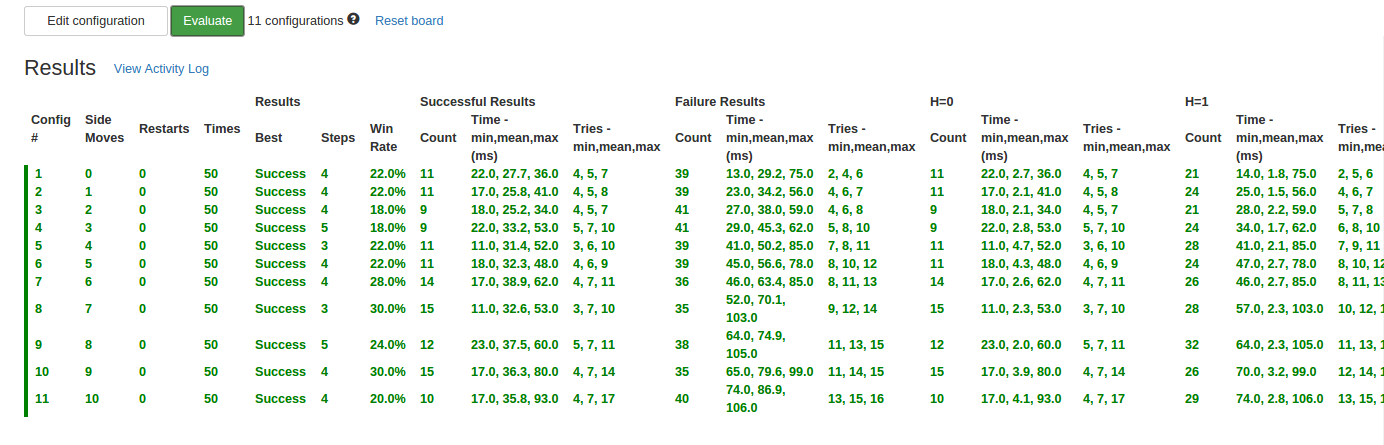
\includegraphics[width=90mm]{img/sideways.png}
\caption{Results showing win rates with sidways moves in the range k=[0:10]. Improvements are not realized until k=6}
\label{fig:ui}
\end{figure}


\subsection{Hill Climbing with Random Restarts}


\subsection{Hill Climbing with Sideways Moves and Random Restarts}


\subsection{Extension: Brute Force via Random Generation}

